\documentclass{article}

% content/resources/templates/preamble.tex
\usepackage[margin=0.6in]{geometry}
\author{Milav Dabgar}
\usepackage{amsmath,amssymb,amsthm}
\usepackage{booktabs}
\usepackage{multirow}
\usepackage{xcolor}
\usepackage{tcolorbox}
\tcbuselibrary{breakable,skins}
\usepackage[colorlinks=true,linkcolor=blue]{hyperref}
\usepackage{titlesec}
\usepackage{enumitem}
\usepackage{tikz}
\usepackage{pgfplots}
\usepackage{circuitikz}
\usepackage[version=4]{mhchem}
\usepackage{longtable}
\usepackage{array}
\usepackage{float}
\usepackage{caption}
\usepackage{listings}

\lstset{
  basicstyle=\small\ttfamily,
  breaklines=true,
  breakatwhitespace=false,
  postbreak=\mbox{\textcolor{red}{$\hookrightarrow$}\space},
  float=false,
  numbers=left,
  numberstyle=\tiny\color{gray},
  numbersep=10pt,
  xleftmargin=2em,
  keywordstyle=\color{blue},
  commentstyle=\color{green!60!black},
  stringstyle=\color{purple},
  backgroundcolor=\color{gray!5},
  showstringspaces=false,
  tabsize=2,
  captionpos=b,
  keepspaces=true,
  columns=flexible
}

\pgfplotsset{compat=1.18}
\usetikzlibrary{shapes,arrows,positioning,calc,patterns,decorations.pathmorphing,decorations.markings,arrows.meta}

% Color scheme
\definecolor{headcolor}{RGB}{0,102,204}
\definecolor{keycolor}{RGB}{220,20,60}
\definecolor{solutioncolor}{RGB}{34,139,34}
\definecolor{mnemoniccolor}{RGB}{148,0,211}
\definecolor{codecolor}{RGB}{0,0,100}

% Spacing
\setlength{\parskip}{3pt}
\setlist[itemize]{nosep}
\setlist[enumerate]{nosep}

% Title formatting
\titleformat{\section}{\Large\bfseries\color{headcolor}}{\thesection}{1em}{}
\titleformat{\subsection}{\large\bfseries\color{headcolor}}{\thesubsection}{1em}{}

% Pandoc tightlist compatibility
\providecommand{\tightlist}{%
  \setlength{\itemsep}{0pt}\setlength{\parskip}{0pt}}

% Pandoc longtable compatibility
\newcounter{none}
\def\thenone{}


% content/resources/templates/english-boxes.tex

% Custom environments
\newtcolorbox{solutionbox}{
 breakable,
 enhanced,
 colback=solutioncolor!5!white,
 colframe=solutioncolor!75!black,
 fonttitle=\bfseries,
 title=Solution
}

\newtcolorbox{solutionboxnobreak}{
 colback=solutioncolor!5!white,
 colframe=solutioncolor!75!black,
 fonttitle=\bfseries,
 title=Solution
}

\newtcolorbox{keyformula}{
 breakable,
 enhanced,
 colback=keycolor!5!white,
 colframe=keycolor!75!black,
 fonttitle=\bfseries,
 title=Key Formula
}

\newtcolorbox{mnemonicboxenv}{
 breakable,
 enhanced,
 colback=mnemoniccolor!5!white,
 colframe=mnemoniccolor!75!black,
 fonttitle=\bfseries,
 title=Mnemonic
}

\newcommand{\mnemonicbox}[1]{%
  \begin{mnemonicboxenv}
    #1
  \end{mnemonicboxenv}
}


% Custom commands for GTU solutions
% This file defines semantic commands for consistent formatting

% Question command with automatic formatting
\newcommand{\question}[2]{%
  \section*{Question #1}%
  \textbf{#2}%
}

% OR question variant
\newcommand{\questionor}[2]{%
  \section*{Question #1 OR}%
  \textbf{#2}%
}

% Proper table environment with caption
\newenvironment{answertable}[1]{%
  \begin{table}[htbp]
  \centering
  \caption{#1}
}{%
  \end{table}
}

% Proper figure environment for diagrams
\newenvironment{answerdiagram}[1]{%
  \begin{figure}[htbp]
  \centering
  \caption{#1}
}{%
  \end{figure}
}

% Semantic markup for key terms
\newcommand{\keyword}[1]{\textbf{#1}}
\newcommand{\code}[1]{\texttt{#1}}
\newcommand{\classname}[1]{\texttt{#1}}
\newcommand{\methodname}[1]{\texttt{#1}}

% Proper quotation marks
\newcommand{\mnemonic}[1]{``#1''}

\usetikzlibrary{fit, trees, positioning}

\title{Linux Operating System (4331602) - Winter 2024 Solution}
\date{December 05, 2024}

\begin{document}
\maketitle

\questionmarks{1(a)}{3}{Explain Multiprogramming Operating System and give its advantages.}

\begin{solutionbox}
\textbf{Answer}:

\textbf{Multiprogramming Operating System} allows multiple programs to reside in memory simultaneously and execute concurrently by sharing CPU time efficiently.

\begin{center}
\captionof{table}{Multiprogramming System Features}
\begin{tabulary}{\linewidth}{|L|L|}
\hline
\textbf{Feature} & \textbf{Description} \\ \hline
\textbf{Memory Management} & Multiple programs loaded in memory \\ \hline
\textbf{CPU Scheduling} & CPU switches between programs \\ \hline
\textbf{Resource Sharing} & Efficient utilization of system resources \\ \hline
\end{tabulary}
\end{center}

\begin{itemize}
    \item \textbf{Increased CPU utilization}: CPU remains busy switching between programs
    \item \textbf{Better throughput}: More programs completed per unit time
    \item \textbf{Reduced response time}: Programs execute faster due to parallel processing
\end{itemize}
\end{solutionbox}

\begin{mnemonicbox}
\mnemonic{MCP - Memory sharing, CPU utilization, Parallel execution}
\end{mnemonicbox}

\questionmarks{1(b)}{4}{Explain Characteristics of Linux operating system.}

\begin{solutionbox}
\textbf{Answer}:

\begin{center}
\captionof{table}{Linux Operating System Characteristics}
\begin{tabulary}{\linewidth}{|L|L|}
\hline
\textbf{Characteristic} & \textbf{Description} \\ \hline
\textbf{Open Source} & Source code freely available and modifiable \\ \hline
\textbf{Multi-user} & Multiple users can access system simultaneously \\ \hline
\textbf{Multi-tasking} & Multiple processes run concurrently \\ \hline
\textbf{Portable} & Runs on various hardware platforms \\ \hline
\textbf{Security} & Strong permission system and access controls \\ \hline
\textbf{Stability} & Robust and reliable system performance \\ \hline
\end{tabulary}
\end{center}

\begin{itemize}
    \item \textbf{Case sensitive}: Distinguishes between uppercase and lowercase
    \item \textbf{Command line interface}: Powerful shell for system operations
    \item \textbf{File system hierarchy}: Organized directory structure starting from root (/)
\end{itemize}
\end{solutionbox}

\begin{mnemonicbox}
\mnemonic{LAMPS - Linux is Accessible, Multi-user, Portable, Secure}
\end{mnemonicbox}

\questionmarks{1(c)}{7}{Explain FCFS scheduling algorithm with its advantages and disadvantages. Calculate Average waiting time and average turnaround time for FCFS algorithm with gantt chart for following data.}

\begin{solutionbox}
\textbf{Answer}:

\textbf{First Come First Serve (FCFS)} is a non-preemptive scheduling algorithm where processes are executed in order of their arrival.

\begin{center}
\captionof{table}{FCFS Algorithm Analysis}
\begin{tabulary}{\linewidth}{|L|L|}
\hline
\textbf{Aspect} & \textbf{Description} \\ \hline
\textbf{Policy} & First arrived process gets CPU first \\ \hline
\textbf{Type} & Non-preemptive \\ \hline
\textbf{Implementation} & Simple queue (FIFO) \\ \hline
\end{tabulary}
\end{center}

\textbf{Advantages:}
\begin{itemize}
    \item \textbf{Simple implementation}: Easy to understand and code
    \item \textbf{Fair scheduling}: No starvation occurs
\end{itemize}

\textbf{Disadvantages:}
\begin{itemize}
    \item \textbf{Convoy effect}: Short processes wait for long processes
    \item \textbf{Poor average waiting time}: Not optimal for system performance
\end{itemize}

\textbf{Gantt Chart Calculation:}
\begin{center}
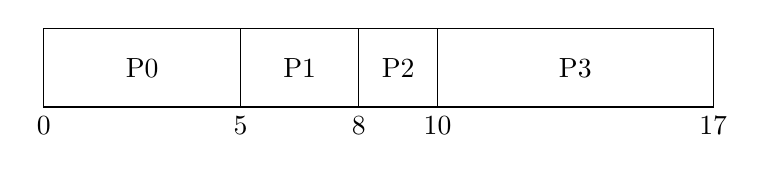
\begin{tikzpicture}[x=0.5cm, y=1cm]
    \draw (0,0) rectangle (5,1) node[midway] {P0};
    \draw (5,0) rectangle (8,1) node[midway] {P1};
    \draw (8,0) rectangle (10,1) node[midway] {P2};
    \draw (10,0) rectangle (17,1) node[midway] {P3};
    
    \node[below] at (0,0) {0};
    \node[below] at (5,0) {5};
    \node[below] at (8,0) {8};
    \node[below] at (10,0) {10};
    \node[below] at (17,0) {17};
\end{tikzpicture}
\captionof{figure}{Gantt Chart (FCFS)}
\end{center}

\begin{center}
\captionof{table}{Process Execution Analysis}
\begin{tabulary}{\linewidth}{|L|L|L|L|L|L|L|}
\hline
\textbf{Process} & \textbf{Arrival} & \textbf{Burst} & \textbf{Start} & \textbf{Finish} & \textbf{Waiting} & \textbf{Turnaround} \\ \hline
P0 & 0 & 5 & 0 & 5 & 0 & 5 \\ \hline
P1 & 3 & 3 & 5 & 8 & 2 & 5 \\ \hline
P2 & 5 & 2 & 8 & 10 & 3 & 5 \\ \hline
P3 & 6 & 7 & 10 & 17 & 4 & 11 \\ \hline
\end{tabulary}
\end{center}

\textbf{Average Waiting Time} = $(0+2+3+4)/4 = \textbf{2.25 ms}$ \\
\textbf{Average Turnaround Time} = $(5+5+5+11)/4 = \textbf{6.5 ms}$
\end{solutionbox}

\begin{mnemonicbox}
\mnemonic{FCFS-SiNo - First Come First Serve is Simple but Not optimal}
\end{mnemonicbox}

\questionmarks{1(c) OR}{7}{Explain Round Robin algorithm with its advantages and disadvantages. Calculate Average waiting time and average turnaround time for Round Robin algorithm with gantt chart for following data. (Time Quantum = 2 ms)}

\begin{solutionbox}
\textbf{Answer}:

\textbf{Round Robin} is a preemptive scheduling algorithm where each process gets equal CPU time slice (quantum).

\begin{center}
\captionof{table}{Round Robin Features}
\begin{tabulary}{\linewidth}{|L|L|}
\hline
\textbf{Feature} & \textbf{Description} \\ \hline
\textbf{Time Quantum} & Fixed time slice for each process \\ \hline
\textbf{Preemption} & Process interrupted after quantum expires \\ \hline
\textbf{Queue Type} & Circular ready queue \\ \hline
\end{tabulary}
\end{center}

\textbf{Advantages:}
\begin{itemize}
    \item \textbf{Fair allocation}: Each process gets equal CPU time
    \item \textbf{No starvation}: All processes eventually get CPU
\end{itemize}

\textbf{Disadvantages:}
\begin{itemize}
    \item \textbf{Context switching overhead}: Frequent process switching
    \item \textbf{Performance depends on quantum}: Too small or large affects efficiency
\end{itemize}

\textbf{Gantt Chart (Quantum = 2ms):}
\begin{center}
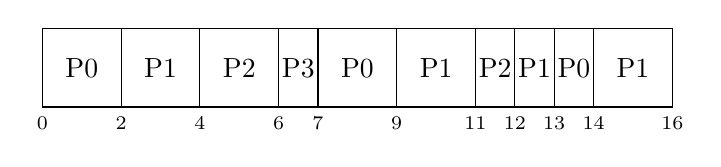
\begin{tikzpicture}[x=0.5cm, y=1cm]
    \draw (0,0) rectangle (2,1) node[midway] {P0};
    \draw (2,0) rectangle (4,1) node[midway] {P1};
    \draw (4,0) rectangle (6,1) node[midway] {P2};
    \draw (6,0) rectangle (7,1) node[midway] {P3};
    \draw (7,0) rectangle (9,1) node[midway] {P0};
    \draw (9,0) rectangle (11,1) node[midway] {P1};
    \draw (11,0) rectangle (12,1) node[midway] {P2};
    \draw (12,0) rectangle (13,1) node[midway] {P1};
    \draw (13,0) rectangle (14,1) node[midway] {P0};
    \draw (14,0) rectangle (16,1) node[midway] {P1};
    
    \foreach \x in {0,2,4,6,7,9,11,12,13,14,16}
        \node[below, font=\scriptsize] at (\x,0) {\x};
\end{tikzpicture}
\captionof{figure}{Gantt Chart (Round Robin)}
\end{center}

\begin{center}
\captionof{table}{Round Robin Execution}
\begin{tabulary}{\linewidth}{|L|L|L|L|L|L|}
\hline
\textbf{Process} & \textbf{Arrival} & \textbf{Burst} & \textbf{Completion} & \textbf{Waiting} & \textbf{Turnaround} \\ \hline
P0 & 0 & 4 & 14 & 10 & 14 \\ \hline
P1 & 1 & 5 & 16 & 10 & 15 \\ \hline
P2 & 2 & 3 & 12 & 7 & 10 \\ \hline
P3 & 3 & 1 & 7 & 3 & 4 \\ \hline
\end{tabulary}
\end{center}

\textbf{Average Waiting Time} = $(10+10+7+3)/4 = \textbf{7.5 ms}$ \\
\textbf{Average Turnaround Time} = $(14+15+10+4)/4 = \textbf{10.75 ms}$
\end{solutionbox}

\begin{mnemonicbox}
\mnemonic{RR-TEQ - Round Robin uses Time Equal Quantum}
\end{mnemonicbox}

\questionmarks{2(a)}{3}{Explain Real Time Operation System.}

\begin{solutionbox}
\textbf{Answer}:

\textbf{Real Time Operating System (RTOS)} processes data and responds to events within strict time constraints.

\begin{center}
\captionof{table}{RTOS Types}
\begin{tabulary}{\linewidth}{|L|L|L|}
\hline
\textbf{Type} & \textbf{Response Time} & \textbf{Example} \\ \hline
\textbf{Hard Real-time} & Guaranteed deadline & Missile guidance \\ \hline
\textbf{Soft Real-time} & Flexible deadline & Video streaming \\ \hline
\end{tabulary}
\end{center}

\begin{itemize}
    \item \textbf{Deterministic behavior}: Predictable response times
    \item \textbf{Priority-based scheduling}: Critical tasks get higher priority
    \item \textbf{Minimal latency}: Fast interrupt handling and context switching
\end{itemize}
\end{solutionbox}

\begin{mnemonicbox}
\mnemonic{RTD - Real Time is Deterministic}
\end{mnemonicbox}

\questionmarks{2(b)}{4}{Explain Process Life Cycle with diagram.}

\begin{solutionbox}
\textbf{Answer}:

\textbf{Process Life Cycle} shows different states a process goes through during execution.

\begin{center}
\begin{tikzpicture}[node distance=2cm, auto]
    \node [gtu state] (new) {New};
    \node [gtu state, right=of new] (ready) {Ready};
    \node [gtu state, right=of ready] (running) {Running};
    \node [gtu state, right=of running] (term) {Terminated};
    \node [gtu state, below=of ready] (wait) {Waiting};

    \path [gtu arrow] (new) -- node {Admit} (ready);
    \path [gtu arrow] (ready) -- node {Dispatch} (running);
    \path [gtu arrow] (running) -- node {Exit} (term);
    \path [gtu arrow] (running) edge [bend right] node [above] {Time Quantum} (ready);
    \path [gtu arrow] (running) -- node {I/O Req} (wait);
    \path [gtu arrow] (wait) -- node {I/O Done} (ready);
\end{tikzpicture}
\captionof{figure}{Process State Transition}
\end{center}

\begin{center}
\captionof{table}{Process States}
\begin{tabulary}{\linewidth}{|L|L|}
\hline
\textbf{State} & \textbf{Description} \\ \hline
\textbf{New} & Process being created \\ \hline
\textbf{Ready} & Waiting for CPU assignment \\ \hline
\textbf{Running} & Instructions being executed \\ \hline
\textbf{Waiting} & Waiting for I/O completion \\ \hline
\textbf{Terminated} & Process finished execution \\ \hline
\end{tabulary}
\end{center}
\end{solutionbox}

\begin{mnemonicbox}
\mnemonic{NRRWT - New Ready Running Waiting Terminated}
\end{mnemonicbox}

\questionmarks{2(c)}{7}{Explain Various file and directory related commands in Linux.}

\begin{solutionbox}
\textbf{Answer}:

\begin{center}
\captionof{table}{File Commands}
\begin{tabulary}{\linewidth}{|L|L|L|}
\hline
\textbf{Command} & \textbf{Function} & \textbf{Example} \\ \hline
\textbf{ls} & List directory contents & \code{ls -la} \\ \hline
\textbf{cat} & Display file content & \code{cat file.txt} \\ \hline
\textbf{cp} & Copy files & \code{cp source dest} \\ \hline
\textbf{mv} & Move/rename files & \code{mv old new} \\ \hline
\textbf{rm} & Remove files & \code{rm file.txt} \\ \hline
\end{tabulary}
\end{center}

\begin{center}
\captionof{table}{Directory Commands}
\begin{tabulary}{\linewidth}{|L|L|L|}
\hline
\textbf{Command} & \textbf{Function} & \textbf{Example} \\ \hline
\textbf{mkdir} & Create directory & \code{mkdir mydir} \\ \hline
\textbf{rmdir} & Remove empty directory & \code{rmdir mydir} \\ \hline
\textbf{cd} & Change directory & \code{cd /home} \\ \hline
\textbf{pwd} & Print working directory & \code{pwd} \\ \hline
\end{tabulary}
\end{center}

\begin{itemize}
    \item \textbf{File permissions}: Use \code{chmod} to modify access rights
    \item \textbf{File ownership}: Use \code{chown} to change file owner
    \item \textbf{File information}: Use \code{stat} for detailed file information
\end{itemize}
\end{solutionbox}

\begin{mnemonicbox}
\mnemonic{LCCMR-MRCP - List, Cat, Copy, Move, Remove for files; Make ...}
\end{mnemonicbox}

\questionmarks{2(a) OR}{3}{Describe operating system services in detail.}

\begin{solutionbox}
\textbf{Answer}:

\textbf{Operating System Services} provide interface between user applications and hardware resources.

\begin{center}
\captionof{table}{OS Services Categories}
\begin{tabulary}{\linewidth}{|L|L|}
\hline
\textbf{Category} & \textbf{Services} \\ \hline
\textbf{User Interface} & GUI, Command Line, Batch \\ \hline
\textbf{Program Execution} & Loading, Running, Terminating \\ \hline
\textbf{I/O Operations} & File operations, Device communication \\ \hline
\textbf{File System} & Creation, Deletion, Manipulation \\ \hline
\textbf{Communication} & Process communication, Network \\ \hline
\textbf{Error Detection} & Hardware/Software error handling \\ \hline
\end{tabulary}
\end{center}

\begin{itemize}
    \item \textbf{Resource allocation}: CPU, memory, and device management
    \item \textbf{Accounting}: Track resource usage and performance
    \item \textbf{Protection and security}: Access control and authentication
\end{itemize}
\end{solutionbox}

\begin{mnemonicbox}
\mnemonic{UPIFCE - User interface, Program execution, I/O, File system, Communication, Error detection}
\end{mnemonicbox}

\questionmarks{2(b) OR}{4}{Explain Process Control Block.}

\begin{solutionbox}
\textbf{Answer}:

\textbf{Process Control Block (PCB)} is a data structure containing all information about a process.

\begin{center}
\captionof{table}{PCB Components}
\begin{tabulary}{\linewidth}{|L|L|}
\hline
\textbf{Component} & \textbf{Information Stored} \\ \hline
\textbf{Process ID} & Unique process identifier \\ \hline
\textbf{Process State} & Current state (ready, running, waiting) \\ \hline
\textbf{CPU Registers} & Program counter, stack pointer, registers \\ \hline
\textbf{Memory Management} & Base/limit registers, page tables \\ \hline
\textbf{I/O Status} & Open files, allocated devices \\ \hline
\textbf{Accounting} & CPU usage, time limits \\ \hline
\end{tabulary}
\end{center}

\begin{center}
\begin{tikzpicture}[node distance=0cm]
    \node [gtu block, minimum width=5cm] (pid) {Process ID};
    \node [gtu block, minimum width=5cm, below=of pid] (state) {Process State};
    \node [gtu block, minimum width=5cm, below=of state] (pc) {Program Counter};
    \node [gtu block, minimum width=5cm, below=of pc] (reg) {CPU Registers};
    \node [gtu block, minimum width=5cm, below=of reg] (mem) {Memory Limits};
    \node [gtu block, minimum width=5cm, below=of mem] (files) {Open File List};
    \node [gtu block, minimum width=5cm, below=of files] (acc) {Accounting Info};
\end{tikzpicture}
\captionof{figure}{PCB Structure}
\end{center}
\end{solutionbox}

\begin{mnemonicbox}
\mnemonic{PPCMIA - Process ID, Process state, Program Counter, CPU registers, Memory, I/O, Accounting}
\end{mnemonicbox}

\questionmarks{2(c) OR}{7}{Explain installation steps of Linux.}

\begin{solutionbox}
\textbf{Answer}:

\textbf{Linux Installation} involves preparing system and installing operating system from bootable media.

\begin{center}
\captionof{table}{Installation Steps}
\begin{tabulary}{\linewidth}{|L|L|}
\hline
\textbf{Step} & \textbf{Description} \\ \hline
\textbf{1. Download ISO} & Get Linux distribution image file \\ \hline
\textbf{2. Create Bootable Media} & Use USB/DVD to create installation media \\ \hline
\textbf{3. Boot from Media} & Change BIOS/UEFI boot order \\ \hline
\textbf{4. Select Language} & Choose installation language \\ \hline
\textbf{5. Partition Disk} & Create root, swap, home partitions \\ \hline
\textbf{6. Configure Network} & Set IP, DNS, hostname \\ \hline
\textbf{7. Create User Account} & Set username, password \\ \hline
\textbf{8. Install Bootloader} & Configure GRUB for booting \\ \hline
\textbf{9. Complete Installation} & Remove media and reboot \\ \hline
\end{tabulary}
\end{center}

\textbf{Partitioning Scheme:}
\begin{itemize}
    \item \textbf{Root (/)}: 20GB minimum for system files
    \item \textbf{Swap}: 2x RAM size for virtual memory
    \item \textbf{Home (/home)}: Remaining space for user data
\end{itemize}

\textbf{Post-installation:}
\begin{itemize}
    \item \textbf{Update system}: \code{sudo apt update \&\& sudo apt upgrade}
    \item \textbf{Install drivers}: Graphics, network, audio drivers
    \item \textbf{Configure security}: Firewall, user permissions
\end{itemize}
\end{solutionbox}

\begin{mnemonicbox}
\mnemonic{DCBSLNCIU - Download, Create media, Boot, Select language, Layout disk, Network, Create user...}
\end{mnemonicbox}

\questionmarks{3(a)}{3}{Define: Process, Program, Swapping}

\begin{solutionbox}
\textbf{Answer}:

\begin{center}
\captionof{table}{Basic Definitions}
\begin{tabulary}{\linewidth}{|L|L|}
\hline
\textbf{Term} & \textbf{Definition} \\ \hline
\textbf{Process} & Program in execution with allocated resources \\ \hline
\textbf{Program} & Set of instructions stored on disk \\ \hline
\textbf{Swapping} & Moving processes between memory and disk \\ \hline
\end{tabulary}
\end{center}

\begin{itemize}
    \item \textbf{Process}: Active entity with process ID, memory space, and execution state
    \item \textbf{Program}: Passive entity, executable file stored in secondary storage
    \item \textbf{Swapping}: Memory management technique to handle more processes than physical memory
\end{itemize}
\end{solutionbox}

\begin{mnemonicbox}
\mnemonic{PAP-MDS - Process is Active Program; Program is instructions; Swapping is Memory-Disk transfer}
\end{mnemonicbox}

\questionmarks{3(b)}{4}{List out various file operations and describe each of them.}

\begin{solutionbox}
\textbf{Answer}:

\begin{center}
\captionof{table}{File Operations}
\begin{tabulary}{\linewidth}{|L|L|L|}
\hline
\textbf{Operation} & \textbf{Description} & \textbf{System Call} \\ \hline
\textbf{Create} & Make new file with specified name & \code{creat()} \\ \hline
\textbf{Open} & Prepare file for reading/writing & \code{open()} \\ \hline
\textbf{Read} & Retrieve data from file & \code{read()} \\ \hline
\textbf{Write} & Store data to file & \code{write()} \\ \hline
\textbf{Close} & Finish file access, release resources & \code{close()} \\ \hline
\textbf{Delete} & Remove file from file system & \code{unlink()} \\ \hline
\textbf{Seek} & Move file pointer to specific position & \code{lseek()} \\ \hline
\end{tabulary}
\end{center}

\begin{itemize}
    \item \textbf{File attributes}: Access permissions, timestamps, size information
    \item \textbf{File locking}: Prevent concurrent access conflicts
    \item \textbf{Buffer management}: Optimize I/O performance through caching
\end{itemize}
\end{solutionbox}

\begin{mnemonicbox}
\mnemonic{CORWCDS - Create, Open, Read, Write, Close, Delete, Seek}
\end{mnemonicbox}

\questionmarks{3(c)}{7}{Write a shell script to generate and print Fibonacci series.}

\begin{solutionbox}
\textbf{Fibonacci Series} generates numbers where each number is sum of two preceding numbers.

\begin{lstlisting}[language=bash, caption={Fibonacci Script}]
#!/bin/bash
# Fibonacci series generator

echo "Enter number of terms:"
read n

a=0
b=1

echo "Fibonacci Series:"
echo -n "$a $b "

for((i=2; i<n; i++))
do
    c=$((a + b))
    echo -n "$c "
    a=$b
    b=$c
done
echo
\end{lstlisting}

\begin{center}
\captionof{table}{Script Components}
\begin{tabulary}{\linewidth}{|L|L|}
\hline
\textbf{Component} & \textbf{Purpose} \\ \hline
\textbf{\#!/bin/bash} & Shebang line specifying interpreter \\ \hline
\textbf{read n} & Accept user input for number of terms \\ \hline
\textbf{for loop} & Iterate to generate sequence \\ \hline
\textbf{Arithmetic} & Calculate next number in series \\ \hline
\end{tabulary}
\end{center}
\end{solutionbox}

\begin{mnemonicbox}
\mnemonic{FLAB - Fibonacci uses Loop with Addition of Both previous numbers}
\end{mnemonicbox}

\questionmarks{3(a) OR}{3}{List out types of scheduler and explain any one of them.}

\begin{solutionbox}
\textbf{Answer}:

\begin{center}
\captionof{table}{Types of Schedulers}
\begin{tabulary}{\linewidth}{|L|L|}
\hline
\textbf{Scheduler Type} & \textbf{Function} \\ \hline
\textbf{Long-term} & Selects processes from job pool to ready queue \\ \hline
\textbf{Short-term} & Selects process from ready queue for CPU \\ \hline
\textbf{Medium-term} & Handles swapping between memory and disk \\ \hline
\end{tabulary}
\end{center}

\textbf{Short-term Scheduler (CPU Scheduler):}
\begin{itemize}
    \item \textbf{Frequency}: Executes very frequently (milliseconds)
    \item \textbf{Function}: Decides which process gets CPU next
    \item \textbf{Algorithms}: FCFS, SJF, Round Robin, Priority
    \item \textbf{Goal}: Maximize CPU utilization and throughput
\end{itemize}
\end{solutionbox}

\begin{mnemonicbox}
\mnemonic{LSM-JRC - Long-term (Job), Short-term (Ready), Medium-term (swap Control)}
\end{mnemonicbox}

\questionmarks{3(b) OR}{4}{List out various file attributes and describe each of them.}

\begin{solutionbox}
\textbf{Answer}:

\begin{center}
\captionof{table}{File Attributes}
\begin{tabulary}{\linewidth}{|L|L|}
\hline
\textbf{Attribute} & \textbf{Description} \\ \hline
\textbf{Name} & Human-readable file identifier \\ \hline
\textbf{Type} & File format (text, binary, executable) \\ \hline
\textbf{Size} & Current file size in bytes \\ \hline
\textbf{Location} & Physical address on storage device \\ \hline
\textbf{Protection} & Access permissions (read, write, execute) \\ \hline
\textbf{Time stamps} & Creation, modification, access times \\ \hline
\textbf{Owner} & User who created the file \\ \hline
\end{tabulary}
\end{center}

\textbf{Permission Structure:}
\begin{itemize}
    \item \textbf{User (u)}: Owner permissions
    \item \textbf{Group (g)}: Group member permissions  
    \item \textbf{Other (o)}: All other users permissions
\end{itemize}
\end{solutionbox}

\begin{mnemonicbox}
\mnemonic{NTSLPTO - Name, Type, Size, Location, Protection, Time, Owner}
\end{mnemonicbox}

\questionmarks{3(c) OR}{7}{Write a shell script to sum of 1 to 10 using while loop.}

\begin{solutionbox}
\textbf{While Loop} continues execution as long as specified condition remains true.

\begin{lstlisting}[language=bash, caption={Sum 1 to 10}]
#!/bin/bash
# Sum of numbers 1 to 10 using while loop

echo "Calculating sum of 1 to 10:"

i=1
sum=0

while [ $i -le 10 ]
do
    sum=$((sum + i))
    echo "Adding $i, current sum: $sum"
    i=$((i + 1))
done

echo "Final sum of 1 to 10 is: $sum"
\end{lstlisting}

\begin{center}
\captionof{table}{Script Logic}
\begin{tabulary}{\linewidth}{|L|L|}
\hline
\textbf{Component} & \textbf{Purpose} \\ \hline
\textbf{i=1} & Initialize counter variable \\ \hline
\textbf{sum=0} & Initialize accumulator \\ \hline
\textbf{while [ \$i -le 10 ]} & Continue while i $\le$ 10 \\ \hline
\textbf{sum=\$((sum + i))} & Add current number to sum \\ \hline
\textbf{i=\$((i + 1))} & Increment counter \\ \hline
\end{tabulary}
\end{center}
\end{solutionbox}

\begin{mnemonicbox}
\mnemonic{WICS - While loop needs Initialize, Condition, Sum calculation}
\end{mnemonicbox}

\questionmarks{4(a)}{3}{List out and explain condition for Deadlock to occur.}

\begin{solutionbox}
\textbf{Answer}:

\textbf{Deadlock} occurs when processes wait indefinitely for resources held by each other.

\begin{center}
\captionof{table}{Deadlock Conditions (Coffman Conditions)}
\begin{tabulary}{\linewidth}{|L|L|}
\hline
\textbf{Condition} & \textbf{Description} \\ \hline
\textbf{Mutual Exclusion} & Only one process can use resource at a time \\ \hline
\textbf{Hold and Wait} & Process holds resources while waiting for others \\ \hline
\textbf{No Preemption} & Resources cannot be forcibly taken away \\ \hline
\textbf{Circular Wait} & Circular chain of processes waiting for resources \\ \hline
\end{tabulary}
\end{center}

\textbf{All four conditions must be true simultaneously for deadlock to occur.}
\end{solutionbox}

\begin{mnemonicbox}
\mnemonic{MHNC - Mutual exclusion, Hold and wait, No preemption, Circular wait}
\end{mnemonicbox}

\questionmarks{4(b)}{4}{List out File access methods. Explain any one.}

\begin{solutionbox}
\textbf{Answer}:

\begin{center}
\captionof{table}{File Access Methods}
\begin{tabulary}{\linewidth}{|L|L|}
\hline
\textbf{Method} & \textbf{Description} \\ \hline
\textbf{Sequential Access} & Read file from beginning to end \\ \hline
\textbf{Direct Access} & Jump to any record directly \\ \hline
\textbf{Index Sequential} & Combination of sequential and indexed access \\ \hline
\end{tabulary}
\end{center}

\textbf{Sequential Access Method:}
\begin{itemize}
    \item \textbf{Process}: Read records one by one in order
    \item \textbf{Advantages}: Simple implementation, efficient for batch processing
    \item \textbf{Disadvantages}: Slow for specific record access
\end{itemize}
\end{solutionbox}

\begin{mnemonicbox}
\mnemonic{SDI - Sequential (start to end), Direct (jump anywhere), Index (combined approach)}
\end{mnemonicbox}

\questionmarks{4(c)}{7}{Describe Security measures in operating system.}

\begin{solutionbox}
\textbf{Answer}:

\textbf{Operating System Security} protects system resources from unauthorized access and threats.

\begin{center}
\captionof{table}{Security Mechanisms}
\begin{tabulary}{\linewidth}{|L|L|}
\hline
\textbf{Mechanism} & \textbf{Description} \\ \hline
\textbf{Authentication} & Verify user identity (passwords, biometrics) \\ \hline
\textbf{Authorization} & Control resource access permissions \\ \hline
\textbf{Access Control Lists} & Define who can access specific resources \\ \hline
\textbf{Encryption} & Protect data confidentiality \\ \hline
\textbf{Audit Logs} & Track system activities and access \\ \hline
\textbf{Firewalls} & Control network traffic \\ \hline
\end{tabulary}
\end{center}

\textbf{Security Levels:}
\begin{itemize}
    \item \textbf{Physical security}: Protect hardware and facilities
    \item \textbf{User authentication}: Login credentials and biometrics
    \item \textbf{File permissions}: Read, write, execute controls
    \item \textbf{Network security}: Secure communication protocols
\end{itemize}
\end{solutionbox}

\begin{mnemonicbox}
\mnemonic{AAAEAF - Authentication, Authorization, Access control, Encryption, Audit, Firewall}
\end{mnemonicbox}

\questionmarks{4(a) OR}{3}{List out ways to deal with deadlock. Explain deadlock detection and recovery.}

\begin{solutionbox}
\textbf{Answer}:

\begin{center}
\captionof{table}{Deadlock Handling Methods}
\begin{tabulary}{\linewidth}{|L|L|}
\hline
\textbf{Method} & \textbf{Approach} \\ \hline
\textbf{Prevention} & Ensure at least one Coffman condition cannot hold \\ \hline
\textbf{Avoidance} & Dynamically examine resource allocation state \\ \hline
\textbf{Detection \& Recovery} & Allow deadlock, then detect and recover \\ \hline
\textbf{Ignore} & Assume deadlock never occurs (Ostrich algorithm) \\ \hline
\end{tabulary}
\end{center}

\textbf{Deadlock Detection:}
\begin{itemize}
    \item \textbf{Wait-for graph}: Maintain graph of process dependencies
    \item \textbf{Detection algorithm}: Periodically check for cycles in graph
\end{itemize}

\textbf{Deadlock Recovery:}
\begin{itemize}
    \item \textbf{Process termination}: Kill one or more deadlocked processes
    \item \textbf{Resource preemption}: Take resources from processes
    \item \textbf{Rollback}: Return processes to safe state using checkpoints
\end{itemize}
\end{solutionbox}

\begin{mnemonicbox}
\mnemonic{PADI - Prevention, Avoidance, Detection, Ignore}
\end{mnemonicbox}

\questionmarks{4(b) OR}{4}{List out File allocation methods. Explain any one.}

\begin{solutionbox}
\textbf{Answer}:

\begin{center}
\captionof{table}{File Allocation Methods}
\begin{tabulary}{\linewidth}{|L|L|}
\hline
\textbf{Method} & \textbf{Description} \\ \hline
\textbf{Contiguous} & Allocate consecutive disk blocks \\ \hline
\textbf{Linked} & Use pointers to link scattered blocks \\ \hline
\textbf{Indexed} & Use index block to store block addresses \\ \hline
\end{tabulary}
\end{center}

\textbf{Contiguous Allocation:}
\begin{itemize}
    \item \textbf{Structure}: File occupies consecutive blocks on disk
    \item \textbf{Advantages}: Fast access, simple implementation, good for sequential access
    \item \textbf{Disadvantages}: External fragmentation, difficult to grow files
    \item \textbf{Directory entry}: Contains starting address and length
\end{itemize}
\end{solutionbox}

\begin{mnemonicbox}
\mnemonic{CLI - Contiguous (consecutive), Linked (pointers), Indexed (table)}
\end{mnemonicbox}

\questionmarks{4(c) OR}{7}{Describe program threats and system threats.}

\begin{solutionbox}
\textbf{Answer}:

\textbf{Program Threats} are malicious software that can harm system or data.

\begin{center}
\captionof{table}{Program Threats}
\begin{tabulary}{\linewidth}{|L|L|}
\hline
\textbf{Threat Type} & \textbf{Description} \\ \hline
\textbf{Virus} & Self-replicating code that infects other programs \\ \hline
\textbf{Worm} & Standalone malware that spreads across networks \\ \hline
\textbf{Trojan Horse} & Malicious code disguised as legitimate software \\ \hline
\textbf{Logic Bomb} & Code that triggers malicious action on specific event \\ \hline
\end{tabulary}
\end{center}

\textbf{System Threats} target operating system and system resources.

\begin{center}
\captionof{table}{System Threats}
\begin{tabulary}{\linewidth}{|L|L|}
\hline
\textbf{Threat Type} & \textbf{Description} \\ \hline
\textbf{Buffer Overflow} & Overflow input buffers to execute malicious code \\ \hline
\textbf{Denial of Service} & Overwhelm system resources to make service unavailable \\ \hline
\textbf{Privilege Escalation} & Gain higher access privileges than authorized \\ \hline
\textbf{Man-in-the-Middle} & Intercept communication between two parties \\ \hline
\end{tabulary}
\end{center}
\end{solutionbox}

\begin{mnemonicbox}
\mnemonic{VWTLB-BPDM - Virus, Worm, Trojan, Logic bomb... Buffer overflow...}
\end{mnemonicbox}

\questionmarks{5(a)}{3}{Explain Inter Process Communication.}

\begin{solutionbox}
\textbf{Answer}:

\textbf{Inter Process Communication (IPC)} enables processes to exchange data and synchronize activities.

\begin{center}
\captionof{table}{IPC Mechanisms}
\begin{tabulary}{\linewidth}{|L|L|}
\hline
\textbf{Mechanism} & \textbf{Description} \\ \hline
\textbf{Pipes} & Unidirectional communication channel \\ \hline
\textbf{Message Queues} & Structured message passing \\ \hline
\textbf{Shared Memory} & Common memory area for multiple processes \\ \hline
\textbf{Semaphores} & Synchronization using counters \\ \hline
\textbf{Signals} & Software interrupts for notification \\ \hline
\end{tabulary}
\end{center}
\end{solutionbox}

\begin{mnemonicbox}
\mnemonic{PMSSS - Pipes, Message queues, Shared memory, Semaphores, Signals}
\end{mnemonicbox}

\questionmarks{5(b)}{4}{Explain File structure used by Linux.}

\begin{solutionbox}
\textbf{Answer}:

\textbf{Linux File System} follows hierarchical directory structure starting from root directory.

\begin{center}
\begin{tikzpicture}[
    node distance=0.5cm,
    every node/.style={gtu block, minimum width=1.5cm, font=\small},
    level 1/.style={sibling distance=2.5cm},
    level 2/.style={sibling distance=1.5cm}
]
    \node {/}
        child {node {bin}
            child {node {ls}}
            child {node {cat}}
        }
        child {node {etc}
            child {node {passwd}}
        }
        child {node {home}
            child {node {user1}
                child {node {Docs}}
            }
        };
\end{tikzpicture}
\captionof{figure}{Linux File System Hierarchy}
\end{center}

\begin{center}
\captionof{table}{Important Directories}
\begin{tabulary}{\linewidth}{|L|L|}
\hline
\textbf{Directory} & \textbf{Purpose} \\ \hline
\textbf{/} & Root directory, top of hierarchy \\ \hline
\textbf{/bin} & Essential user commands \\ \hline
\textbf{/etc} & System configuration files \\ \hline
\textbf{/home} & User home directories \\ \hline
\textbf{/var} & Variable data (logs, mail) \\ \hline
\textbf{/usr} & User programs and utilities \\ \hline
\textbf{/tmp} & Temporary files \\ \hline
\end{tabulary}
\end{center}
\end{solutionbox}

\begin{mnemonicbox}
\mnemonic{BEHVUT - Bin, Etc, Home, Var, Usr, Tmp}
\end{mnemonicbox}

\questionmarks{5(c)}{7}{Explain operating system security policies and procedures.}

\begin{solutionbox}
\textbf{Answer}:

\textbf{Security Policies} define rules and guidelines for protecting system resources and data.

\begin{center}
\captionof{table}{Security Policy Components}
\begin{tabulary}{\linewidth}{|L|L|}
\hline
\textbf{Component} & \textbf{Description} \\ \hline
\textbf{Access Control Policy} & Who can access what resources \\ \hline
\textbf{Password Policy} & Requirements for strong passwords \\ \hline
\textbf{Audit Policy} & What activities to monitor and log \\ \hline
\textbf{Backup Policy} & Data backup and recovery procedures \\ \hline
\textbf{Incident Response} & Steps to handle security breaches \\ \hline
\end{tabulary}
\end{center}

\textbf{Security Procedures:}
\begin{itemize}
    \item \textbf{Authentication}: Multi-factor authentication, Password complexity
    \item \textbf{Authorization}: Principle of least privilege, Role-based access
    \item \textbf{Monitoring}: Log analysis, Intrusion detection
\end{itemize}
\end{solutionbox}

\begin{mnemonicbox}
\mnemonic{APABI - Access control, Password, Audit, Backup, Incident response}
\end{mnemonicbox}

\questionmarks{5(a) OR}{3}{Explain Critical section.}

\begin{solutionbox}
\textbf{Answer}:

\textbf{Critical Section} is code segment where process accesses shared resources that must not be accessed concurrently.

\begin{center}
\captionof{table}{Critical Section Properties}
\begin{tabulary}{\linewidth}{|L|L|}
\hline
\textbf{Property} & \textbf{Description} \\ \hline
\textbf{Mutual Exclusion} & Only one process in critical section at a time \\ \hline
\textbf{Progress} & Selection of next process cannot be postponed indefinitely \\ \hline
\textbf{Bounded Waiting} & Limit on number of times other processes enter critical section \\ \hline
\end{tabulary}
\end{center}

\textbf{Structure:}
\begin{lstlisting}[basicstyle=\ttfamily]
do {
    entry_section();     // Request permission
    critical_section();  // Access shared resource
    exit_section();      // Release permission
    remainder_section(); // Other work
} while(true);
\end{lstlisting}
\end{solutionbox}

\begin{mnemonicbox}
\mnemonic{MPB - Mutual exclusion, Progress, Bounded waiting}
\end{mnemonicbox}

\questionmarks{5(b) OR}{4}{Explain types of Linux file system.}

\begin{solutionbox}
\textbf{Answer}:

\textbf{Linux File Systems} organize and manage data storage on disk devices.

\begin{center}
\captionof{table}{Linux File System Types}
\begin{tabulary}{\linewidth}{|L|L|}
\hline
\textbf{File System} & \textbf{Description} \\ \hline
\textbf{ext4} & Fourth extended file system, most common \\ \hline
\textbf{XFS} & High-performance journaling file system \\ \hline
\textbf{Btrfs} & B-tree file system with advanced features \\ \hline
\textbf{ZFS} & Zettabyte file system with built-in RAID \\ \hline
\end{tabulary}
\end{center}

\textbf{ext4 Features:}
\begin{itemize}
    \item \textbf{Journaling}: Faster recovery after system crash
    \item \textbf{Large file support}: Files up to 16TB
    \item \textbf{Backwards compatibility}: Can mount ext2/ext3 partitions
\end{itemize}
\end{solutionbox}

\begin{mnemonicbox}
\mnemonic{EXBZNF - Ext4, XFS, Btrfs, ZFS, NTFS, FAT32}
\end{mnemonicbox}

\questionmarks{5(c) OR}{7}{Explain need of protection mechanism and various protection domain.}

\begin{solutionbox}
\textbf{Answer}:

\textbf{Protection Mechanism} prevents processes from interfering with each other and system resources.

\textbf{Need for Protection:}
\begin{itemize}
    \item \textbf{Resource sharing}: Multiple users/processes access same resources
    \item \textbf{Error containment}: Prevent bugs from affecting entire system
    \item \textbf{Security enforcement}: Implement access control policies
\end{itemize}

\begin{center}
\captionof{table}{Protection Domains}
\begin{tabulary}{\linewidth}{|L|L|}
\hline
\textbf{Domain Type} & \textbf{Description} \\ \hline
\textbf{User Domain} & Limited access rights for user processes \\ \hline
\textbf{Kernel Domain} & Full access to system resources \\ \hline
\textbf{System Domain} & Intermediate privileges for system services \\ \hline
\end{tabulary}
\end{center}

\begin{center}
\captionof{table}{Access Rights}
\begin{tabulary}{\linewidth}{|L|L|}
\hline
\textbf{Right} & \textbf{Description} \\ \hline
\textbf{Read} & View content of resource \\ \hline
\textbf{Write} & Modify resource content \\ \hline
\textbf{Execute} & Run program or enter directory \\ \hline
\end{tabulary}
\end{center}
\end{solutionbox}

\begin{mnemonicbox}
\mnemonic{RECES-UKS - Resource sharing, Error containment, Security; User domain, Kernel domain...}
\end{mnemonicbox}

\end{document}
